The Top control region ($\crtop$) is used to estimate the contribution of
$t \bar{t}$ and single top processes in the signal region. It is defined in the
same way as the $\crwmn$ control region defined in \cref{sec:muon-cr-bveto} but
at least one $b$-jet is required instead of the veto. \cref{fig:top_plots}
report the $\met$ and the leading jet $\pt$ distributions after the background
only fit described in \cref{sec:glob-simult-likel,sec:fit-strategy}. It shows,
within uncertainties, a good agreement between data and \gls{mc}.
\begin{figure}[!th]
  \centering
  \begin{subfigure}[t]{.48\linewidth}
    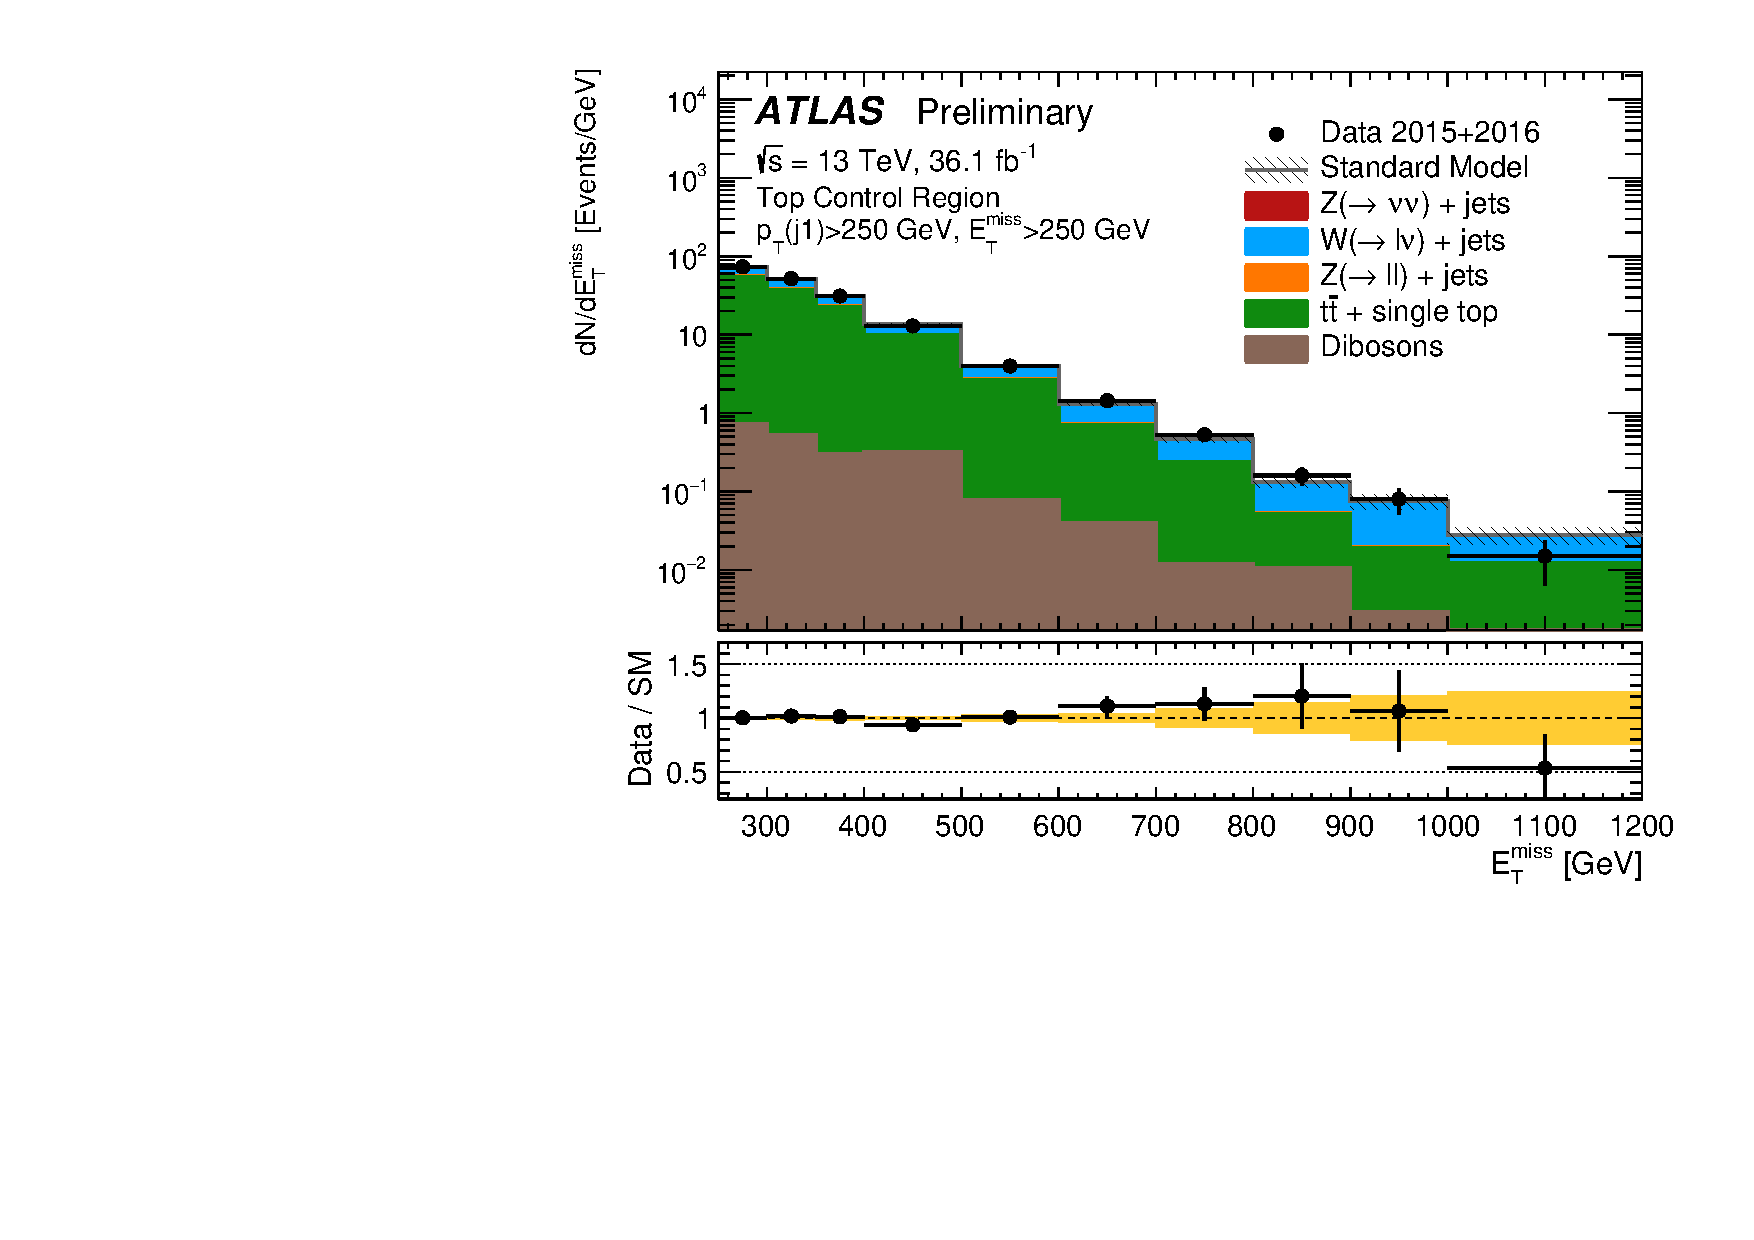
\includegraphics[width=\linewidth]{top_cr_met}
    \caption{$\met$ distribution.}
    \label{fig:top_cr_et_miss}
  \end{subfigure}
  \begin{subfigure}[t]{.48\linewidth}
    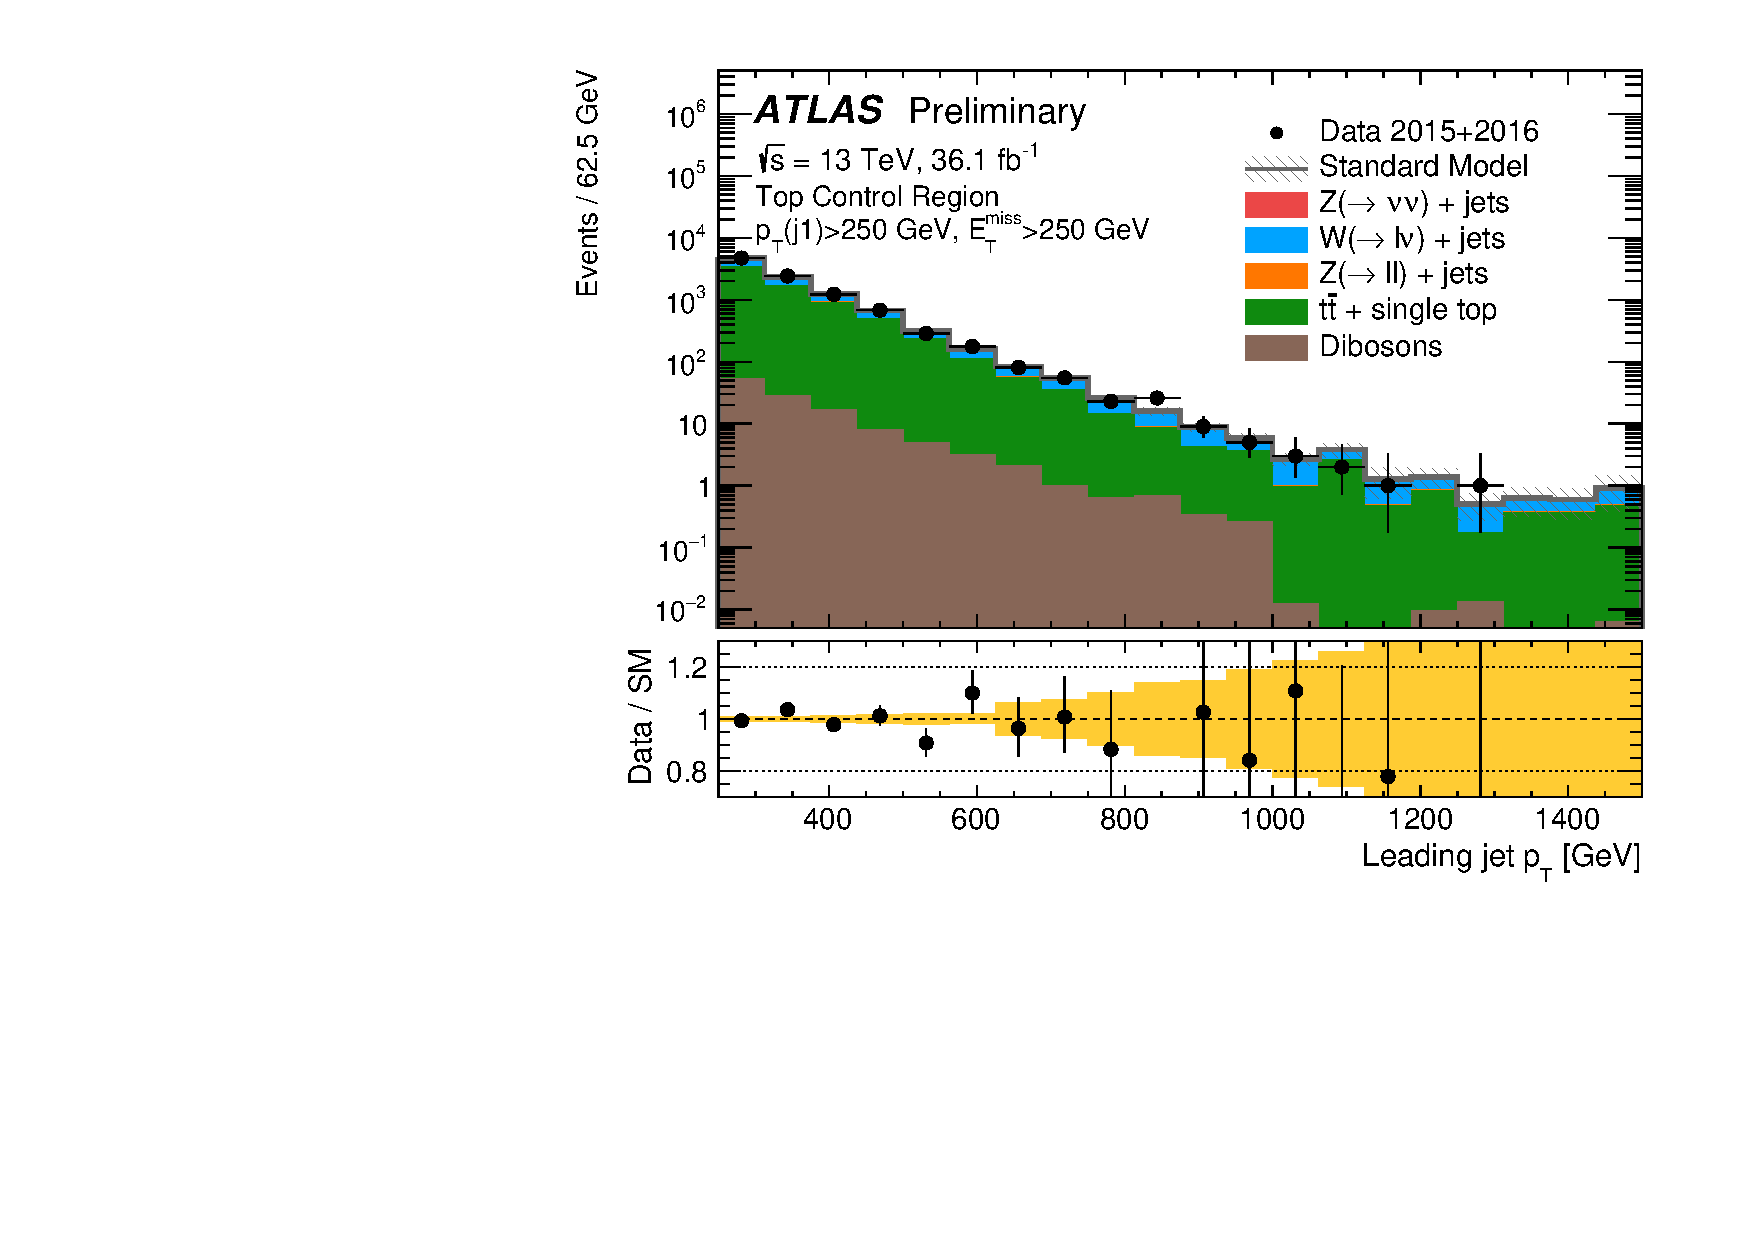
\includegraphics[width=\linewidth]{top_cr_jet1}
    \caption{Leading jet $\pt$ distribution.}
    \label{fig:top_cr_jet1}
  \end{subfigure}
  \caption{Observed and predicted $\met$ and leading jet $\pt$ after the
    background only fit in the $\crtop$ control region for the $\met > 250$~GeV
    inclusive selection. The error bands in the ratio plot on the bottom of the
    figures include statistical and systematic uncertainties. The negligible
    contribution of \gls{ncb} and diboson backgrounds is not reported in the
    figure.}
  \label{fig:top_plots}
\end{figure}
%%% Local Variables:
%%% mode: latex
%%% TeX-master: "../search_for_DM_LED_with_ATLAS"
%%% End:
